%main.tex
%Found report example at overleaf example section: 
%(https://www.overleaf.com/articles/clustering-the-interstellar-medium/mtthgyyfrdkn#.VdSUtR_ithE)
%http://www.latextemplates.com/template/the-legrand-orange-book
%%%%%%%%%%%%%%%%%%%%%%%%%%%%%%%%%%%%%%%%%
%  My documentation report
%  Objetive: Explain what I did and how, so someone can continue with the investigation
%
% Important note:
% Chapter heading images should have a 2:1 width:height ratio,
% e.g. 920px width and 460px height.
%
%%%%%%%%%%%%%%%%%%%%%%%%%%%%%%%%%%%%%%%%%

%----------------------------------------------------------------------------------------
%	PACKAGES AND OTHER DOCUMENT CONFIGURATIONS
%----------------------------------------------------------------------------------------

\documentclass[11pt,fleqn]{book} % Default font size and left-justified equations

\usepackage[top=3cm,bottom=3cm,left=3.2cm,right=3.2cm,headsep=10pt,letterpaper]{geometry} % Page margins

\usepackage{xcolor} % Required for specifying colors by name
\definecolor{ocre}{RGB}{52,177,201} % Define the orange color used for highlighting throughout the book

\usepackage{comment}

% Font Settings
\usepackage{avant} % Use the Avantgarde font for headings
%\usepackage{times} % Use the Times font for headings
\usepackage{mathptmx} % Use the Adobe Times Roman as the default text font together with math symbols from the Sym­bol, Chancery and Com­puter Modern fonts

\usepackage{microtype} % Slightly tweak font spacing for aesthetics
\usepackage[utf8]{inputenc} % Required for including letters with accents
\usepackage[T1]{fontenc} % Use 8-bit encoding that has 256 glyphs

% Bibliography
\usepackage[style=alphabetic,sorting=nyt,sortcites=true,autopunct=true,babel=hyphen,hyperref=true,abbreviate=false,backref=true,backend=biber]{biblatex}
\addbibresource{bibliography.bib} % BibTeX bibliography file
\defbibheading{bibempty}{}

%----------------------------------------------------------------------------------------
%	VARIOUS REQUIRED PACKAGES
%----------------------------------------------------------------------------------------

\usepackage{titlesec} % Allows customization of titles

\usepackage{graphicx} % Required for including pictures
\graphicspath{{Pictures/}} % Specifies the directory where pictures are stored
\usepackage{hyperref}

\usepackage{lipsum} % Inserts dummy text
\usepackage{listings}

\definecolor{codegreen}{rgb}{0,0.6,0}
\definecolor{codegray}{rgb}{0.5,0.5,0.5}
\definecolor{codepurple}{rgb}{0.58,0,0.82}
\definecolor{backcolour}{rgb}{0.95,0.95,0.92}
\definecolor{lightblue}{rgb}{0.35,0.65,0.92}
\lstdefinestyle{Python}{
    backgroundcolor=\color{backcolour},   
    commentstyle=\color{codegreen},
    keywordstyle=\color{magenta},
    numberstyle=\tiny\color{codegray},
    stringstyle=\color{codepurple},
    basicstyle=\footnotesize,
    breakatwhitespace=false,      
    breaklines=true,
    captionpos=b,
    keepspaces=true,
    numbers=left,                    
    numbersep=5pt,                  
    showspaces=false,                
    showstringspaces=false,
    showtabs=false,                  
    tabsize=2,
    keepspaces=true, 
    columns=flexible
}








\usepackage{tikz} % Required for drawing custom shapes

\usepackage[english]{babel} % English language/hyphenation

\usepackage{enumitem} % Customize lists
\setlist{nolistsep} % Reduce spacing between bullet points and numbered lists

\usepackage{booktabs} % Required for nicer horizontal rules in tables

\usepackage{eso-pic} % Required for specifying an image background in the title page

%----------------------------------------------------------------------------------------
%	MAIN TABLE OF CONTENTS
%----------------------------------------------------------------------------------------

\usepackage{titletoc} % Required for manipulating the table of contents

\contentsmargin{0cm} % Removes the default margin
% Chapter text styling
\titlecontents{chapter}[1.25cm] % Indentation
{\addvspace{15pt}\large\sffamily\bfseries} % Spacing and font options for chapters
{\color{ocre!60}\contentslabel[\Large\thecontentslabel]{1.25cm}\color{ocre}} % Chapter number
{}  
{\color{ocre!60}\normalsize\sffamily\bfseries\;\titlerule*[.5pc]{.}\;\thecontentspage} % Page number
% Section text styling
\titlecontents{section}[1.25cm] % Indentation
{\addvspace{5pt}\sffamily\bfseries} % Spacing and font options for sections
{\contentslabel[\thecontentslabel]{1.25cm}} % Section number
{}
{\sffamily\hfill\color{black}\thecontentspage} % Page number
[]
% Subsection text styling
\titlecontents{subsection}[1.25cm] % Indentation
{\addvspace{1pt}\sffamily\small} % Spacing and font options for subsections
{\contentslabel[\thecontentslabel]{1.25cm}} % Subsection number
{}
{\sffamily\;\titlerule*[.5pc]{.}\;\thecontentspage} % Page number
[] 

%----------------------------------------------------------------------------------------
%	MINI TABLE OF CONTENTS IN CHAPTER HEADS
%----------------------------------------------------------------------------------------

% Section text styling
\titlecontents{lsection}[0em] % Indendating
{\footnotesize\sffamily} % Font settings
{}
{}
{}

% Subsection text styling
\titlecontents{lsubsection}[.5em] % Indentation
{\normalfont\footnotesize\sffamily} % Font settings
{}
{}
{}
 
%----------------------------------------------------------------------------------------
%	PAGE HEADERS
%----------------------------------------------------------------------------------------

\usepackage{fancyhdr} % Required for header and footer configuration



\pagestyle{fancy}
\renewcommand{\chaptermark}[1]{\markboth{\sffamily\normalsize\bfseries\chaptername\ \thechapter.\ #1}{}} % Chapter text font settings
\renewcommand{\sectionmark}[1]{\markright{\sffamily\normalsize\thesection\hspace{5pt}#1}{}} % Section text font settings
\fancyhf{} \fancyhead[LE,RO]{\sffamily\normalsize\thepage} % Font setting for the page number in the header
\fancyhead[LO]{\rightmark} % Print the nearest section name on the left side of odd pages
\fancyhead[RE]{\leftmark} % Print the current chapter name on the right side of even pages
\renewcommand{\headrulewidth}{0.5pt} % Width of the rule under the header
\addtolength{\headheight}{2.5pt} % Increase the spacing around the header slightly
\renewcommand{\footrulewidth}{0pt} % Removes the rule in the footer
\fancypagestyle{plain}{\fancyhead{}\renewcommand{\headrulewidth}{0pt}} % Style for when a plain pagestyle is specified

% Removes the header from odd empty pages at the end of chapters
\makeatletter
\renewcommand{\cleardoublepage}{
\clearpage\ifodd\c@page\else
\hbox{}
\vspace*{\fill}
\thispagestyle{empty}
\newpage
\fi}

%----------------------------------------------------------------------------------------
%	THEOREM STYLES
%----------------------------------------------------------------------------------------

\usepackage{amsmath,amsfonts,amssymb,amsthm} % For math equations, theorems, symbols, etc

\newcommand{\intoo}[2]{\mathopen{]}#1\,;#2\mathclose{[}}
\newcommand{\ud}{\mathop{\mathrm{{}d}}\mathopen{}}
\newcommand{\intff}[2]{\mathopen{[}#1\,;#2\mathclose{]}}
\newtheorem{notation}{Notation}[chapter]

%%%%%%%%%%%%%%%%%%%%%%%%%%%%%%%%%%%%%%%%%%%%%%%%%%%%%%%%%%%%%%%%%%%%%%%%%%%
%%%%%%%%%%%%%%%%%%%% dedicated to boxed/framed environements %%%%%%%%%%%%%%
%%%%%%%%%%%%%%%%%%%%%%%%%%%%%%%%%%%%%%%%%%%%%%%%%%%%%%%%%%%%%%%%%%%%%%%%%%%
\newtheoremstyle{ocrenumbox}% % Theorem style name
{0pt}% Space above
{0pt}% Space below
{\normalfont}% % Body font
{}% Indent amount
{\small\bf\sffamily\color{ocre}}% % Theorem head font
{\;}% Punctuation after theorem head
{0.25em}% Space after theorem head
{\small\sffamily\color{ocre}\thmname{#1}\nobreakspace\thmnumber{\@ifnotempty{#1}{}\@upn{#2}}% Theorem text (e.g. Theorem 2.1)
\thmnote{\nobreakspace\the\thm@notefont\sffamily\bfseries\color{black}---\nobreakspace#3.}} % Optional theorem note
\renewcommand{\qedsymbol}{$\blacksquare$}% Optional qed square

\newtheoremstyle{blacknumex}% Theorem style name
{5pt}% Space above
{5pt}% Space below
{\normalfont}% Body font
{} % Indent amount
{\small\bf\sffamily}% Theorem head font
{\;}% Punctuation after theorem head
{0.25em}% Space after theorem head
{\small\sffamily{\tiny\ensuremath{\blacksquare}}\nobreakspace\thmname{#1}\nobreakspace\thmnumber{\@ifnotempty{#1}{}\@upn{#2}}% Theorem text (e.g. Theorem 2.1)
\thmnote{\nobreakspace\the\thm@notefont\sffamily\bfseries---\nobreakspace#3.}}% Optional theorem note

\newtheoremstyle{blacknumbox} % Theorem style name
{0pt}% Space above
{0pt}% Space below
{\normalfont}% Body font
{}% Indent amount
{\small\bf\sffamily}% Theorem head font
{\;}% Punctuation after theorem head
{0.25em}% Space after theorem head
{\small\sffamily\thmname{#1}\nobreakspace\thmnumber{\@ifnotempty{#1}{}\@upn{#2}}% Theorem text (e.g. Theorem 2.1)
\thmnote{\nobreakspace\the\thm@notefont\sffamily\bfseries---\nobreakspace#3.}}% Optional theorem note

%%%%%%%%%%%%%%%%%%%%%%%%%%%%%%%%%%%%%%%%%%%%%%%%%%%%%%%%%%%%%%%%%%%%%%%%%%%
%%%%%%%%%%%%% dedicated to non-boxed/non-framed environements %%%%%%%%%%%%%
%%%%%%%%%%%%%%%%%%%%%%%%%%%%%%%%%%%%%%%%%%%%%%%%%%%%%%%%%%%%%%%%%%%%%%%%%%%
\newtheoremstyle{ocrenum}% % Theorem style name
{5pt}% Space above
{5pt}% Space below
{\normalfont}% % Body font
{}% Indent amount
{\small\bf\sffamily\color{ocre}}% % Theorem head font
{\;}% Punctuation after theorem head
{0.25em}% Space after theorem head
{\small\sffamily\color{ocre}\thmname{#1}\nobreakspace\thmnumber{\@ifnotempty{#1}{}\@upn{#2}}% Theorem text (e.g. Theorem 2.1)
\thmnote{\nobreakspace\the\thm@notefont\sffamily\bfseries\color{black}---\nobreakspace#3.}} % Optional theorem note
\renewcommand{\qedsymbol}{$\blacksquare$}% Optional qed square
\makeatother

% Defines the theorem text style for each type of theorem to one of the three styles above
\newcounter{dummy} 
\numberwithin{dummy}{section}
\theoremstyle{ocrenumbox}
\newtheorem{theoremeT}[dummy]{Theorem}
\newtheorem{problem}{Problem}[chapter]
\newtheorem{exerciseT}{Exercise}[chapter]
\theoremstyle{blacknumex}
\newtheorem{exampleT}{Example}[chapter]
\theoremstyle{blacknumbox}
\newtheorem{vocabulary}{Vocabulary}[chapter]
\newtheorem{definitionT}{Definition}[section]
\newtheorem{corollaryT}[dummy]{Corollary}
\theoremstyle{ocrenum}
\newtheorem{proposition}[dummy]{Proposition}

%----------------------------------------------------------------------------------------
%	DEFINITION OF COLORED BOXES
%----------------------------------------------------------------------------------------

\RequirePackage[framemethod=default]{mdframed} % Required for creating the theorem, definition, exercise and corollary boxes

% Theorem box
\newmdenv[skipabove=7pt,
skipbelow=7pt,
backgroundcolor=black!5,
linecolor=ocre,
innerleftmargin=5pt,
innerrightmargin=5pt,
innertopmargin=5pt,
leftmargin=0cm,
rightmargin=0cm,
innerbottommargin=5pt]{tBox}

% Exercise box	  
\newmdenv[skipabove=7pt,
skipbelow=7pt,
rightline=false,
leftline=true,
topline=false,
bottomline=false,
backgroundcolor=ocre!10,
linecolor=ocre,
innerleftmargin=5pt,
innerrightmargin=5pt,
innertopmargin=5pt,
innerbottommargin=5pt,
leftmargin=0cm,
rightmargin=0cm,
linewidth=4pt]{eBox}	

% Definition box
\newmdenv[skipabove=7pt,
skipbelow=7pt,
rightline=false,
leftline=true,
topline=false,
bottomline=false,
linecolor=ocre,
innerleftmargin=5pt,
innerrightmargin=5pt,
innertopmargin=0pt,
leftmargin=0cm,
rightmargin=0cm,
linewidth=4pt,
innerbottommargin=0pt]{dBox}	

% Corollary box
\newmdenv[skipabove=7pt,
skipbelow=7pt,
rightline=false,
leftline=true,
topline=false,
bottomline=false,
linecolor=gray,
backgroundcolor=black!5,
innerleftmargin=5pt,
innerrightmargin=5pt,
innertopmargin=5pt,
leftmargin=0cm,
rightmargin=0cm,
linewidth=4pt,
innerbottommargin=5pt]{cBox}

% Creates an environment for each type of theorem and assigns it a theorem text style from the "Theorem Styles" section above and a colored box from above
\newenvironment{theorem}{\begin{tBox}\begin{theoremeT}}{\end{theoremeT}\end{tBox}}
\newenvironment{exercise}{\begin{eBox}\begin{exerciseT}}{\hfill{\color{ocre}\tiny\ensuremath{\blacksquare}}\end{exerciseT}\end{eBox}}				  
\newenvironment{definition}{\begin{dBox}\begin{definitionT}}{\end{definitionT}\end{dBox}}	
\newenvironment{example}{\begin{exampleT}}{\hfill{\tiny\ensuremath{\blacksquare}}\end{exampleT}}		
\newenvironment{corollary}{\begin{cBox}\begin{corollaryT}}{\end{corollaryT}\end{cBox}}	

%----------------------------------------------------------------------------------------
%	REMARK ENVIRONMENT
%----------------------------------------------------------------------------------------

\newenvironment{remark}{\par\vspace{10pt}\small % Vertical white space above the remark and smaller font size
\begin{list}{}{
\leftmargin=35pt % Indentation on the left
\rightmargin=25pt}\item\ignorespaces % Indentation on the right
\makebox[-2.5pt]{\begin{tikzpicture}[overlay]
\node[draw=ocre!60,line width=1pt,circle,fill=ocre!25,font=\sffamily\bfseries,inner sep=2pt,outer sep=0pt] at (-15pt,0pt){\textcolor{ocre}{R}};\end{tikzpicture}} % Orange R in a circle
\advance\baselineskip -1pt}{\end{list}\vskip5pt} % Tighter line spacing and white space after remark

%----------------------------------------------------------------------------------------
%	SECTION NUMBERING IN THE MARGIN
%----------------------------------------------------------------------------------------

\makeatletter
\renewcommand{\@seccntformat}[1]{\llap{\textcolor{ocre}{\csname the#1\endcsname}\hspace{1em}}}                    
\renewcommand{\section}{\@startsection{section}{1}{\z@}
{-4ex \@plus -1ex \@minus -.4ex}
{1ex \@plus.2ex }
{\normalfont\large\sffamily\bfseries}}
\renewcommand{\subsection}{\@startsection {subsection}{2}{\z@}
{-3ex \@plus -0.1ex \@minus -.4ex}
{0.5ex \@plus.2ex }
{\normalfont\sffamily\bfseries}}
\renewcommand{\subsubsection}{\@startsection {subsubsection}{3}{\z@}
{-2ex \@plus -0.1ex \@minus -.2ex}
{.2ex \@plus.2ex }
{\normalfont\small\sffamily\bfseries}}                        
\renewcommand\paragraph{\@startsection{paragraph}{4}{\z@}
{-2ex \@plus-.2ex \@minus .2ex}
{.1ex}
{\normalfont\small\sffamily\bfseries}}

%----------------------------------------------------------------------------------------
%	HYPERLINKS IN THE DOCUMENTS
%----------------------------------------------------------------------------------------

% For an unclear reason, the package should be loaded now and not later
\usepackage{hyperref}
\hypersetup{hidelinks,backref=true,pagebackref=true,hyperindex=true,colorlinks=false,breaklinks=true,urlcolor= ocre,bookmarks=true,bookmarksopen=false,pdftitle={Title},pdfauthor={Author}}

%----------------------------------------------------------------------------------------
%	CHAPTER HEADINGS
%----------------------------------------------------------------------------------------

% The set-up below should be (sadly) manually adapted to the overall margin page septup controlled by the geometry package loaded in the main.tex document. It is possible to implement below the dimensions used in the goemetry package (top,bottom,left,right)... TO BE DONE

\newcommand{\thechapterimage}{}
\newcommand{\chapterimage}[1]{\renewcommand{\thechapterimage}{#1}}

% Numbered chapters with mini tableofcontents
\def\thechapter{\arabic{chapter}}
\def\@makechapterhead#1{
\thispagestyle{empty}
{\centering \normalfont\sffamily
\ifnum \c@secnumdepth >\m@ne
\if@mainmatter
\startcontents
\begin{tikzpicture}[remember picture,overlay]
\node at (current page.north west)
{\begin{tikzpicture}[remember picture,overlay]
\node[anchor=north west,inner sep=0pt] at (0,0) {\includegraphics[width=\paperwidth]{\thechapterimage}};
%%%%%%%%%%%%%%%%%%%%%%%%%%%%%%%%%%%%%%%%%%%%%%%%%%%%%%%%%%%%%%%%%%%%%%%%%%%%%%%%%%%%%
% Commenting the 3 lines below removes the small contents box in the chapter heading
%\fill[color=ocre!10!white,opacity=.6] (1cm,0) rectangle (8cm,-7cm);
%\node[anchor=north west] at (1.1cm,.35cm) {\parbox[t][8cm][t]{6.5cm}{\huge\bfseries\flushleft \printcontents{l}{1}{\setcounter{tocdepth}{2}}}};
\draw[anchor=west] (5cm,-9cm) node [rounded corners=20pt,fill=ocre!10!white,text opacity=1,draw=ocre,draw opacity=1,line width=1.5pt,fill opacity=.6,inner sep=12pt]{\huge\sffamily\bfseries\textcolor{black}{\thechapter. #1\strut\makebox[22cm]{}}};
%%%%%%%%%%%%%%%%%%%%%%%%%%%%%%%%%%%%%%%%%%%%%%%%%%%%%%%%%%%%%%%%%%%%%%%%%%%%%%%%%%%%%
\end{tikzpicture}};
\end{tikzpicture}}
\par\vspace*{230\p@}
\fi
\fi}

% Unnumbered chapters without mini tableofcontents (could be added though) 
\def\@makeschapterhead#1{
\thispagestyle{empty}
{\centering \normalfont\sffamily
\ifnum \c@secnumdepth >\m@ne
\if@mainmatter
\begin{tikzpicture}[remember picture,overlay]
\node at (current page.north west)
{\begin{tikzpicture}[remember picture,overlay]
\node[anchor=north west,inner sep=0pt] at (0,0) {\includegraphics[width=\paperwidth]{\thechapterimage}};
\draw[anchor=west] (5cm,-9cm) node [rounded corners=20pt,fill=ocre!10!white,fill opacity=.6,inner sep=12pt,text opacity=1,draw=ocre,draw opacity=1,line width=1.5pt]{\huge\sffamily\bfseries\textcolor{black}{#1\strut\makebox[22cm]{}}};
\end{tikzpicture}};
\end{tikzpicture}}
\par\vspace*{230\p@}
\fi
\fi
}
\makeatother
 % Insert the commands.tex file which contains the majority of the structure behind the template

\begin{document}

%----------------------------------------------------------------------------------------
%	TITLE PAGE
%----------------------------------------------------------------------------------------

\begingroup
\thispagestyle{empty}
%\AddToShipoutPicture*{\put(0,0){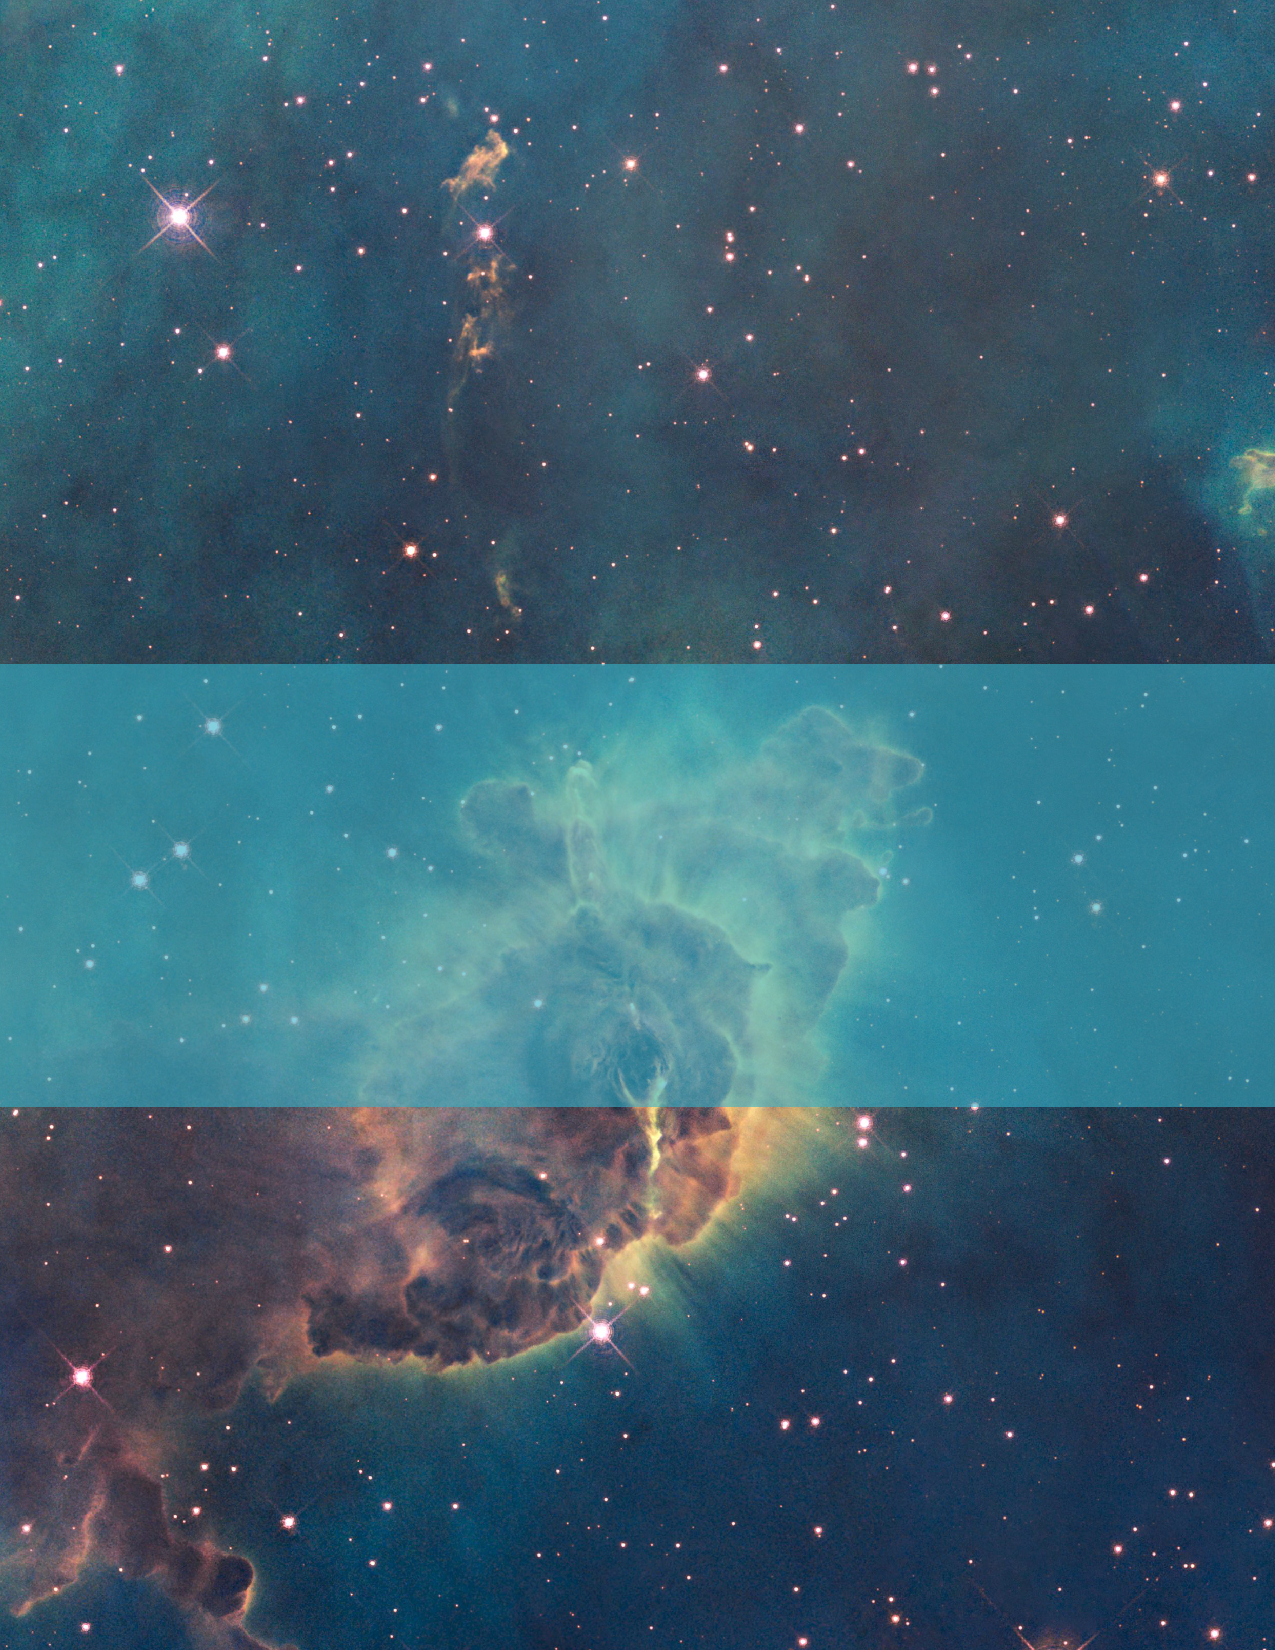
\includegraphics[scale=1.25]{esahubble}}} % Image background

\AddToShipoutPicture*{\put(0,0){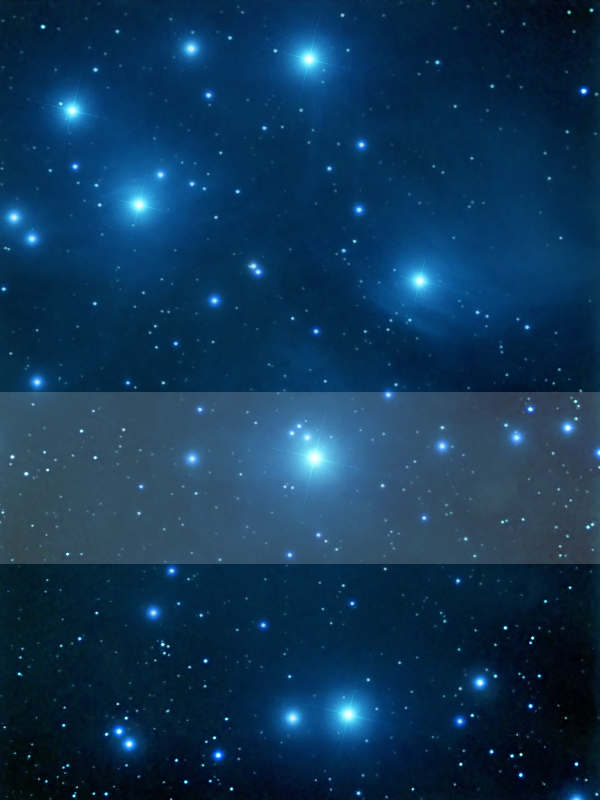
\includegraphics[scale=1.25]{M45grande}}} % Image background
\centering
\vspace*{7cm}
\par\normalfont\fontsize{35}{35}\sffamily\selectfont
\textbf{aLIGO-wxPython}\\
{\LARGE Graphical User Interface for Gravitational Wave Data Analysis}\par % Book title
\vspace*{1cm}
{\Huge Manuel Pichardo Marcano}\par % Author name
\endgroup

%----------------------------------------------------------------------------------------
%	COPYRIGHT PAGE
%----------------------------------------------------------------------------------------

\newpage
~\vfill
\thispagestyle{empty}


\noindent \textsc{Summer Research Project, University of Glasgow}\\

\noindent \textsc{\href{https://github.com/manuelmarcano22/aLIGO-wxPython}{https://github.com/manuelmarcano22/aLIGO-wxPython  }  }\\ % URL

\noindent This research was done under the supervision of Dr. Martin Hendry from June 18th to August 25th of 2015.\\ % License information

\noindent \textit{First release, August 2015} % Printing/edition date

%----------------------------------------------------------------------------------------
%	TABLE OF CONTENTS
%----------------------------------------------------------------------------------------

%\chapterimage{head2.png} % Table of contents heading image
\chapterimage{Helix2.png} % Table of contents heading image

\pagestyle{empty} % No headers

\tableofcontents % Print the table of contents itself
%\lstlistoflistings

%\cleardoublepage % Forces the first chapter to start on an odd page so it's on the right

\pagestyle{fancy} % Print headers again

%----------------------------------------------------------------------------------------
%	CHAPTER 1
%----------------------------------------------------------------------------------------

\begin{comment}
\chapterimage{Perseo2.png} % Chapter heading image

\chapter{Introduction}

\section{Motivation}\index{Motivation}
When I applied for the summer research internship
\begin{quote}
Blah blah
\end{quote}


\begin{remark}
	Instead of having a long bibliography I will write in each chapter the links and books that were useful and deal with the chapter topic. 
\end{remark}

\end{comment}

%------------------------------------------------

%\subsection{References}\index{References}
%
%Since I found so much good information about pretty much everything I wanted to know about, I will just create a remark and let you know where you can find more specific information about, just like below.
%
%\begin{remark}
%For more information about the cosmological principle, review Chapter 1: Why Learn Astronomy?, page 10, from \textbf{21st Century Astronomy}, \textit{Hester | Smith | Blumenthal | Kay | Voss}, Third Edition, 2010.
%\end{remark}

%This statement requires citation \cite{book_key}; this one is more specific \cite[122]{article_key}.


%----------------------------------------------------------------------------------------
%	CHAPTER 2
%----------------------------------------------------------------------------------------
%\chapterimage{band1.png}
\chapterimage{M452.png}

\chapter{The Essentials}

\section{Python}\index{python}

\subsection{Why Python?}


Python is a widely use programming language. The community is a very active and growing one. It is free and open-source software with many open, popular libraries of scientific tools. Some of the most used ones being SciPy \footnote{http://www.scipy.org/}, NumPy \footnote{http://www.numpy.org/}, Matplotlib \footnote{http://matplotlib.org/} and Astropy \footnote{http://www.astropy.org/} . Besides these general reasons, there are other good Python resources more specific to Gravitational Waves data analysis. Three of them are described below:

\vspace{.3 cm}

\begin{description}
	\item[\href{https://losc.ligo.org/tutorials/}{LIGO Open Science Center:}] It provides an introduction to LIGO data files. The webpage provides a number of Python scripts to learn to download and plot actual LIGO data. The tutorials, including the first on how to install the necesarry programs, scripts and plot gallery can be accessed from the page \url{https://losc.ligo.org/tutorials/}.

		\vspace{.3 cm}

\item[\href{https://gwpy.github.io/}{GWpy:}] GWpy is a Python package with "tools and methods for studying data from gravitational waves detectors. The page \url{https://gwpy.github.io/} provides instructions for installation and short tutorial on its use. 

\item[\href{https://www.lsc-group.phys.uwm.edu/daswg/projects/lalsuite.html}{LALSuite}:] LALSuite is maintain by the LIGO Scientific Collaboration Research Group (LSC). It is "compromised of various gravitational wave data analysis routines written in C." I can be installed as a RPM, Dev or from the Git repository. Instruction on how to install: \url{https://www.lsc-group.phys.uwm.edu/daswg/docs/howto/lal-install.html}. Installing from the Git repository didnt prove to be too difficult, but knowing these web resources were useful in the process:
	

	\vspace{.2 cm}
	\begin{description}
		\item[Softaware prerequistes: ] This pages provides a step-by-step instruction to install the LSC software required for the LALSuite libraries and tools. (\url{https://www.lsc-group.phys.uwm.edu/daswg/docs/howto/lscsoft-install.html}). Just make sure to install the right version. The page apparently is a bit old and I had a trouble when building LALSuite and had to installed a newer version. Also had a problem when running the ./configure for libmetaio. One solution was to comment out a line as was explain in this installation notes (\url{http://www.ph.unimelb.edu.au/~cchung/installnotes.pdf}). Also had to put on my .bashrc the line 
			\begin{verbatim}
		export PKG_CONFIG=/usr/bin/pkg-config
		\end{verbatim}
		I was having the same problem mentioned in this forum (\url{http://ubuntuforums.org/archive/index.php/t-2217198.html})\\ 
	\begin{description}
		
	\item[SWIG:] is an open source software tool used to connect computer programs or libraries written in C. To be able to use the LALSuite routines in Python when configuring LALSuite to install it need to include the prefix for swig-python:\\ 
        	\begin{verbatim}
		$ ./configure --prefix=${LALSUITE_PREFIX} --enable-swig-python
            \end{verbatim}
	\end{description}

        \end{description}
	\end{description}


\begin{remark}
	Besides the two LSC step-by-step instructios to install LALSuite and the LSC softwares, I list other pages that at some point on the installatin process of LALSuite routines were useful:
	\begin{itemize}	
	\item Problem with \emph{./configure} for lal : \url{http://peekaboo-vision.blogspot.ca/2012/09/segmentation-algorithms-in-scikits-image.html}
	\item Building LIGO's Global Diagnostic System (GDS): Useful installing Frame Library and other dependencies. \url{http://www.spy-hill.net/~myers/help/ligo/GDS-build.html#framecpp}

	\item Christine Chung LSC installation notes: \url{http://www.ph.unimelb.edu.au/~cchung/installnotes.pdf}
	\item \url{http://smirshekari.wikidot.com/lal}
    \end{itemize}
\end{remark}


\subsection{The Python Must have}


As stated above Python have many packages and libraries for many different purposes. The ones that I found essentials while working on the GUI were the following:

\vspace{.5 cm}
\begin{description}
    
        \item[Packages:] \hfill
        	\\
        These ones can be easily installed from the command line using the Python Package Index (PyPI). PyPI is a great tool to install the most up-to-date version of many python packages. It can be install from the command line on a Debian and Ubuntu machine running:
        \begin{verbatim}
        	$ sudo apt-get install python-pip
        \end{verbatim}
        	
        %\begin{itemize}
		\item \textbf{Astropy} contains tools to handle coordinate systems, units, and many more things useful for research in astronomy and astrophysics. I used it to change from gps time to local sidereal time on the observatories. \url{http://www.astropy.org/}
		\item \textbf{Numpy} is a wonderful package to work with arrays. This tutorial is a great way to start learning about the powerful \emph{Numpy arrays}. \url{http://wiki.scipy.org/Tentative_NumPy_Tutorial}.
		\item \textbf{SciPy} have user-friendly and efficient numerical methods routines. \url{http://www.scipy.org/}.
		\item \textbf{Matplotlib.} It is a very powerful tool to visualize data. A gallery with examples and the source code can be found here \url{http://matplotlib.org/}. Also the power of matplotlib can be extended using add-on toolkits. A toolkit for plotting 2D data on maps is called \textbf{Basemap} (http://matplotlib.org/basemap/).
         %   \end{itemize}
\end{description}

\section{wxPython: The GUI toolkit}

wxPython is wrapper of a cross platform GUI library written in C$++$, wxWidgets. wxPython like wxWidgets is open source and cross-paltform. Its initial release was in 1988. So wxPython has been for a long time. This and the fact that there are many resources online makes wxPython a good choice to develope a GUI using Python. 



\begin{remark}
	A great resource to start working in wxPython was the book written by one of its developers Robin Dunn. The book publish by \emph{Manning Publications} in 2006 is called \href{http://www.manning.com/rappin/}{\textbf{wxPython in action}}.

\end{remark}







%----------------------------------------------------------------------------------------
%	CHAPTER 3
%----------------------------------------------------------------------------------------

\chapterimage{Veil2.png}


\chapter{The Theory}


The quest for  gravitational waves started a while ago with the efforts of Joseph Weber. The first gravitational wave detectors where so called 'Weber bars' or resonant bar detectors. The idea was simple, to try to detect the waves by trying to measure the vibrations of the metal bar due to the in passing gravitational waves. There are still some functioning bar detectors around the world with great improve in sensitivities since the mid-60s. Recently the focus have to try to interferometers observatories, ground and space based interferometers. By examining closely the interference pattern of these couples of kilometers long interferometers higher sensitivities can be achieved and these observatories are the ones that  will probable detect the first gravitational waves. In this report we will only focus and discuss the peculiarities of these type of detectors.\\ 


The challenge is hard, but the final goal remains: to be able to directly detected them and see the universe through a complete new window. To quantify detection and detectability a useful concept is the Signal-to-Noise Ratio (SNR). To calculated it we need to know about the source waveform, detectors antenna pattern and understand the different noise sources.\\

The subsequent sections will describe what we mean by SNR in the GW astronomy context, and explore in some detail what we need to know to calculated it. This approached was chosen since it will require  to learn about waveform from compact binaries and its evolution, about different noise sources for different generations of interferometers, antenna patterns, power spectral density, and network of detectors.\\ 

\section{Signal-to-Noise Ratio (SNR)}

We first need to define what we mean by Signal-to-noise ratio. The ideal signal-to-noise ratio, $\rho$, characterizes the detectability of a signal in a detector with a given noise power spectrum. It is defined as :

\begin{equation}\label{eq:rho}
	\rho = \sqrt{4 \, \int^{fmax} _{fmin} \frac{\text{\~ h}^{*}(f) \, \text{\~ h}(f)}{S(f)} df}
\end{equation}



%In this equation we introduced two new variables: h and S. 

where $\text{\~ h}(f)$ is the Fourier transform of the quantity h  called the \emph{Characteristic strain}. The strain amplitude is a dimensionless quantity representing the amplitude of a gravitational wave. It gives the fractional change in displacement between two nearby masses due to the gravitational wave. The $^*$ denotes the complex conjugate. Gravitational radiation has two independent polarization states, $+$ and $\times$, and h is actually a linear combination of the two states, $\, h^2 = h_{+}^2 + h_{\times}^2$. How we can calculate the gravitational wave strain h from a source like a compact binary coalescence is discussed in the next subsection~\ref{sec:waveform}.\\

The other variable introduced was $S(f)$. $\, S(f)$ is the detector power spectral density. The square-root of the power spectral density, $S^{1/2}(f)$, is known as the \emph{amplitude strain densitivity} or \emph{amplitude spectral density (ASD)}.  It has unit of $ [ \text{Hz}^{-1/2} ] $. This would be important when we discuss noise sources and how to get the ASD from all the noise sources in sec~\ref{sec:noise}.







\begin{comment}
\begin{equation}
	h_f = \sqrt{5 \times \pi / 24.}\times G^2 \times M_{chirp}^2/(c^5 \times Dist)\times (\frac{\pi \times G \times M_{chirp} \times fI}{c^3})^{-7./6.}
\end{equation}

The goal and quantifible. 

Waveform

detector: antenna

Noise

Source: ra ande dec and distance
\end{comment}


\section{The Waveform}\label{sec:waveform}


As we saw in the last section we can characterize the strength of a know signal in a detector by the quantity $\rho$ using equation~\ref{eq:rho}. The next question is how we can calculate h?\\

A lot of research have been made in this area to try to simulate and find the analytical expression from different gravitational waves sources (continuous, burst and coalescence). The strain, h, is time dependent but for simplicity we can work entirely on the frequency space. Different sources have different expressions for the characteristic strain, here using the quadrapole and stationary phase approximation we can calculate the real part of the strain in the frequency domain for a binary system in optimal location and orientation at a distance as:

\begin{equation}\label{eq:strain}
	\text{\~h}(f) = \left ( \frac{5 \pi}{24} \right )^{1/2}  \frac{G^2 \mathcal M ^2}{c^5 D} \left ( \pi G \mathcal M  f /c^3 \right )^{-7/6} 
\end{equation}


where $\mathcal M = \mu^{3/5} \, M_{\text{total}}^{2/5} $ ($\mu= M_1*M_2 / M_{\text{total}}$ being the reduced mass) is the \emph{chirp mass},  D is the \emph{luminosity distance}.\\

This is the expression we will use to calculate the SNR of a source with a given chirp mass and at a given distance.  \\

With LALSuite routines installed we can generate different kind of waveforms in the frequency domain. An example using lalsimulation in python to generate the plus and cross polarization components for non-spinning binaries is:

\begin{lstlisting}[language= Python,style=Python,caption={Frequency domain non-spinning inspiral waveform
}]
def fdwaveform(phiref, deltaF, m1, m2, fmin, fmax, dist, incl):
ampO = 0   # 0 pN order in amplitude
phaseO = 7 # 3.5 pN order in phase
approx = lalsimulation.TaylorF2 # Taylor F2 approximant
fref = fmin

hptilde, hctilde = lalsimulation.SimInspiralChooseFDWaveform(phiref, deltaF,
m1*lal.MSUN_SI, m2*lal.MSUN_SI, 0., 0., 0., 0., 0., 0., fmin,
fmax, fref, dist*1e6*lal.PC_SI, incl, 0., 0., None, None, ampO, phaseO, approx)

# return the frequency domain plus and cross waveforms
return hptilde.data.data, hctilde.data.data
\end{lstlisting}



%$$a_{\text{ISCO}} = 6 G M / c^2$$


%Eq. 26 de Schutz http://arxiv.org/pdf/1102.5421.pdf de dependency of inclination called binary radiation pattern. 

\section{Detectors}

Now that we now how the signal looks like in the frequency domain we need to look at the Detectors response to the gravitational wave, and what limit its response. The specific examples on how to calculate the ASD and main source noises of a detector would be discussed only for a second generation one, but it applies also for the other generations. 

%We will only talk about the second generation detectors and only the main noise sources. 

\subsection{Evolution}

\vspace{.3 cm}
\subsubsection{First Generation}
\vspace{.3 cm}

This consist of 5 different observatories in three different continents. iLIGO (initial LIGO) and then eLIGO (enhanced LIGO) in Hanford and Livingston in the USA. Virgo in Italy, GEO 600 in Germany and TAMA 300 in Japan.  For the analytical formulas of the noises for eLIGO see Appendix A.2 of \emph{Creigton and Anderson} \textbf{Gravitational-Wave Physics and Astronomy} by WILEY publisher. It approximate values for parameters of the 4 km ideal initial LIGO and discusses the main source noises. There are also C routines part of lalsimulation to calculate the noises and ASD for eLIGO and other first generation detectors. \href{https://ligo-vcs.phys.uwm.edu/cgit/lalsuite/tree/lalsimulation/src/LALSimNoisePSD.c}{Click here to see the list of the functions}. See listing \ref{lst:psd} in the next subsection for an example on using one of those functions part of lalsimulation in Python to calculate the ASD for two second generation detector, aLIGO and AdvVirgo. \\



\subsubsection{Second Generation}
\vspace{.3 cm}


Second generations include the two Advanced LIGO (aLIGO), Advanced Virgo and the Kamiola Gravitational Wave Detector (KAGRA). This last one was formerly the Large Cryogenic Gravitational Wave Telescope (LCGT). \\

As for the first generation we can use lalsimulation routines if we wish to generate the sensitivity curves and different noises for aLIGO and other second generation detectors. The list of the C routines to generate the different noise curves can be found in this webpage: \url{https://ligo-vcs.phys.uwm.edu/cgit/lalsuite/tree/lalsimulation/src/LALSimNoisePSD.c}. Two examples using those routines in Python would be:\\

\begin{lstlisting}[language= Python,style=Python,caption={Noise power spectrum for aLIGO and AdvVirgo},label={lst:psd}]
import lalsimulation
import lal
import numpy as np

[...]

#First way
#Create a FrequencySeries type: 
psd = lal.CreateREAL8FrequencySeries('name', t0, 0., deltaF, lal.Unit(), len(hp)) # to hold psd
ret = lalsimulation.SimNoisePSDaLIGODesignSensitivityP1200087(psd, fmin)
psd.data.data[psd.data.data == 0.] = np.inf
asd = np.sqrt(psd.data.data) # convert PSD to ASD

#A more straight forward way for AdvVirgo:
freqrange = np.linspace(fmin, fmax, len(datapoints))
asd = np.zeros(len(freqrange))
for i in np.arange(len(freqrange)):
	asd[i] = lalsimulation.SimNoisePSDAdvVirgo(freqrange[i])
asd = np.sqrt(asd)

[...]
\end{lstlisting}

Where \emph{CreateREAL8FrequencySeries} creates a frequency spectrum of data sampled over uniform frequency intervals. As it says in the documentation it includes extra fields "defining the sample frequencies, the timestamp of the spectrum, and the type of data being sampled." The arguments are the name of the data series, the start time of the time series in \href{http://software.ligo.org/docs/lalsuite/lal/struct_l_i_g_o_time_g_p_s.html}{LIGOTimeGPS}, the lowest frequency being sampled, in Hertz, the frequency sampling interval, in Hertz, and the physical units of the quantity being sampled. \href{http://software.ligo.org/docs/lalsuite/lal/group___l_a_l_datatypes.html#ss_FrequencySeries}{Click here for the documentation about the function}. In the second way of doing it we simply evaluate the function \emph{SimNoisePSDAdvVirgo} for every desired frequency.





\subsubsection{Third Generation and Space-borne Observatories }
\vspace{.3 cm}

\begin{itemize}
	\item Einstein Telescope
	\item LISA Path finder and eLISA
\end{itemize}

\subsection{Antenna Pattern}

We can do it in two ways of doing it. An example code to do this in Python is in the \href{https://github.com/manuelmarcano22/aLIGO-wxPython}{git repository}  of the GUI \href{https://github.com/manuelmarcano22/aLIGO-wxPython/blob/master/antennamod.py}{here}. We can also use a routine from lal to get the antenna pattern. Such a function on Python would look like:\\


\begin{lstlisting}[language= Python,style=Python,caption={Antenna Response of a detector},label={lst:antenna}]

def antenna_response( gpsTime, ra, dec, psi, det ):
gps = lal.LIGOTimeGPS( gpsTime )
gmst_rad = lal.GreenwichMeanSiderealTime(gps)

# create detector-name map
detMap = {'H1': lal.LALDetectorIndexLHODIFF, \
	'H2': lal.LALDetectorIndexLHODIFF, \
	'L1': lal.LALDetectorIndexLLODIFF, \
	'G1': lal.LALDetectorIndexGEO600DIFF, \
	'V1': lal.LALDetectorIndexVIRGODIFF, \
	'T1': lal.LALDetectorIndexTAMA300DIFF}

try:
detector=detMap[det]
except KeyError:
raise ValueError, "ERROR. Key %s is not a valid detector name." % (det)

# get detector
detval = lal.CachedDetectors[detector]

response = detval.response

# actual computation of antenna factors
fp, fc = lal.ComputeDetAMResponse(response, ra, dec, psi, gmst_rad)

return fp, fc

\end{lstlisting}

The function defined above returns the beam pattern responses to the plus and cross polarization status of the gravitational waves. We see from the listing above that for each detector it depends on the time, position of the source in the sky and polarization angle. In theory it is frequency dependent too but in the long-wavelength limit the bean pattern functions become frequency-independent. 


\begin{remark}
Antenna pattern for different detectors and networks  see Figure 6 of \href{http://scholarworks.montana.edu/xmlui/bitstream/handle/1/1740/LittenbergT0509.pdf?sequence=1}{A Comprehensive Bayesian Approach to Gravitational Wave Astronomy}\\

Also Chapter 6 of \emph{Creighton and Anderson} \textbf{Gravitational-Wave Physics and Astronomy} by WILEY.
\end{remark}

\subsection{Main Noise Sources}\label{sec:noise}


\vspace{.3 cm}
\subsubsection{Seismic}
\vspace{.3 cm}



\vspace{.3 cm}
\subsubsection{Thermal Noise}
\vspace{.3 cm}

\begin{itemize}
\item Suspension Thermal Noise
\item Coating Brownian Noise
\end{itemize}



\vspace{.3 cm}
\subsubsection{Quantum Noise}
\vspace{.3 cm}




\section{Sky Source}

{\large Earth-fixed coordinate system}

We can convert Right Ascension (ra) and Declination (dec) in the sky of the source at a given epoch to an Earth-fixed coordinate system. 


\section{Network}

To get the average network SNR we add SNR of the individual detectors in quadrature. For example, for a network of two detectors the average SNR of the network, $\rho_{\text{net}}$, can be calculated doing:

\begin{equation}
	<\rho_{\text{net}}> = \sqrt{\rho_{1} ^2 + \rho_{2}^2}
\end{equation}


The  \emph{network antenna pattern} $P_N$ is simply:

\begin{equation}
	P_N = \sum _I R_I P_I
\end{equation}

where $R_I$ is the \emph{sensitivity ratio} for the $I$ detector. If we choose a arbitrary a  reference detector $ref$ we compute $R_I$ as:

\begin{equation}
R_I = \frac{\int ^ {+ \infty} _ {- \infty} df \frac{|h(f)|^2}{S_I(f)}} {\int ^ {+ \infty} _ {- \infty} df \frac{|h(f)|^2}{S_{ref}(f)}} 
\end{equation}

The integral are simply the SNR for each detector. 



\begin{remark}
	\begin{itemize}
		\item A great website with a plot of some sensitivities plot and a paper in arXiv explain in the graph and all about the sensitivity curves is \href{http://arxiv.org/abs/1408.0740}{Gravitational Wave Sensitivity Curve Plotter}\\
	\item Another great is the lectures and exercises of the \href{www.algo.com}{Caltech Gravitational Wave Summer School}. Specially the ipython notebook from the Dr. Weinstein.\\
	\item Book on the subject: \emph{Creigton and Anderson} \textbf{Gravitational-Wave Physics and Astronomy} by WILEY publisher.\\ 

	\item For Network of detectors: \emph{L. Wen and Schutz} discussion on chapter 5 of \textbf{Advanced Gravitational Wave Detectors} edited by David G. Blair.

\end{itemize}
\end{remark}


{\large \textbf{TO DO}}
\begin{itemize}
	\item Extend Third Generation discussion and Noises
	\item More benefit Network like sky position
\end{itemize}


%----------------------------------------------------------------------------------------
%	CHAPTER 4
%----------------------------------------------------------------------------------------

\chapterimage{M42.png} % Chapter heading image
\chapter{Real Noise}


\section{Quadruple Suspension Design for Advanced LIGO}

The routines part of lalsimulation are only approximation and theoretical models. To have a more realistic SNR calculations for aLIGO  we need more accurate representation of the noises. \\

For the fist prototype of the GUI we will only consider the effect of changing the suspension design parameters on the SNR of a particular source. Dr. Giles Hammond and Ms Kyung Ha lee, both at the University of Glasgow, generated data for four different noises. Each data set is a $4500 \times 10$ .txt file that is read into the program to calculate the SNR for a given suspension configuration. aLIGO has a quadruple suspension and we can change three important things on the Suspension of the interferometer.The possible configurations for the three design parameters that we can change are:\\

\begin{itemize}
	\item Total mass of the suspension. 9 possible masses from 40 kg to 120 kg.
	\item Total length. 3 possible configurations (1.6, 1.87 and 2.14 meters).
	\item Sections length (ribbons). Also 3 possibilities (0.6, 0.85 and 1.1 meters). \\
\end{itemize}



{\large \textbf{TO DO}}
\begin{itemize}
	\item Ask Dr. Hammond and Kyung-Ha Lee on detail on computed data
	\item photo or diagram of the suspension 
\end{itemize}

\begin{remark}
	\begin{itemize}
		\item \url{http://labcit.ligo.caltech.edu/docs/public_html/public/P/P020001-A/P020001-A.pdf}
	\end{itemize}
\end{remark}

%----------------------------------------------------------------------------------------
%	CHAPTER 5
%----------------------------------------------------------------------------------------

\chapterimage{Veil2.png}

\chapter{The GUI}

%\section{Graphical User Interface for Gravitational Wave Data Analysis}
\section{Putting it all together}

For an specific compact binary system of the same mass and at a given distance it calculates the Signal-to-Noise Ratio, Horizon Distance. Average Range, Time to innermost stable circular orbits (ISCO), and Time in view for three different detectors configuration (LIGO Hanford, LIGO Livingston and a Network of the two detectors). Three design parameters can be change: 1-Total Suspension Length, 2- Section Suspension Length and 3-Total mass of the suspension. Can select from 9 different masses, and 3 lengths for both the total and section length. Four source parameters can be changed: 1-Mass of the two binaries, 2-Distance of the binaries, 3-Position in the Sky (in Earth-fixed coordinates), 4-Maximun gravitational wave (GW) frequency (GW freq. is twice the orbital frequency). It plots and calculate the amplitude spectral density (ASD) from the Seismic, Suspension Thermal, Coating Brownian and Quantum Noise.\\

The code assumes polarization angle of 0.343, observation time at $t_0=9\times 10^8$ (gps sec), and inclination of 0 (best scenario). It is a stationary phase approximation.

\section{Assumptions}

Stationary phase approximation. The code assumes polarization angle of 0.343, observation time at t0=9e8 (gps sec), and inclination of 0 (best scenario). Assumes no spinning binaries in a circular orbit. 

\section{Future Work}

\begin{itemize}
	\item Include gravity gradient noise
	\item Include time as parameter
	\item More data points for the sliders
	\item Include contribution to SNR beyond the ISCO
	\item Inclination as parameter or randomize
	\item Include eccentric and spinning binaries
\end{itemize}


\begin{figure}[p]
    \centering
    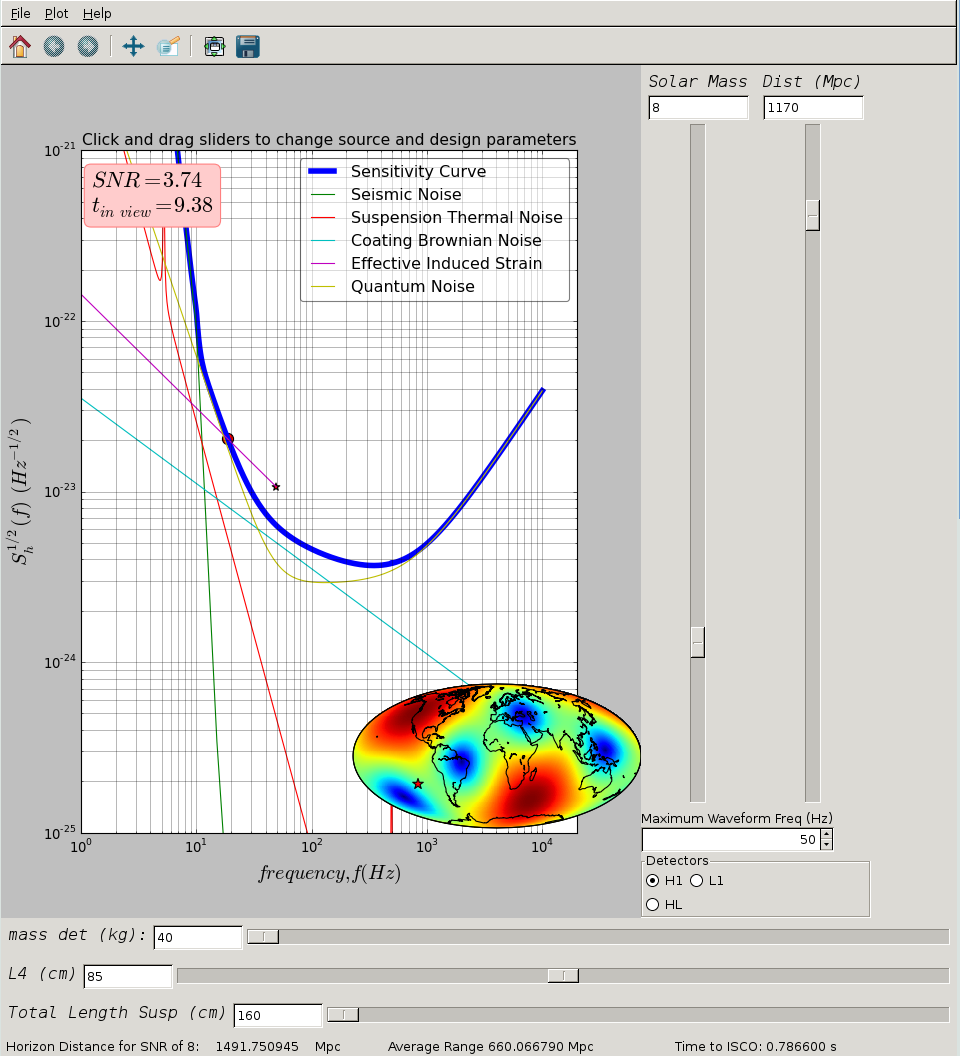
\includegraphics[width=0.8\textwidth]{screenshot5.png}
    \caption{GNU screenshot}
    \label{fig:awesome_image}
\end{figure}




%{\large Dudaddadadadadda en http://arxiv.org/pdf/1102.5421.pdf es 1.16 en abstract de thresgol?}

\end{document}
%main.tex
